\documentclass{beamer}

\mode<presentation>
{
  \usetheme{default}      % or try Darmstadt, Madrid, Warsaw, ...
  \usecolortheme{default} % or try albatross, beaver, crane, ...
  \usefonttheme{default}  % or try serif, structurebold, ...
  \setbeamertemplate{navigation symbols}{}
  \setbeamertemplate{caption}[numbered]
} 

\usepackage[english]{babel}
\usepackage[utf8x]{inputenc}
\setlength\tabcolsep{1.5pt}

\begin{document}
\frame{
\frametitle{Contents}
\tableofcontents
}

\section{Estimation from a damage function}
\frame{
\frametitle{Introductory thoughts}

\begin{itemize}
\item The impact of CO$_2$ on impacts has a much shorter half-life than of CO$_2$ in the atmosphere because of adaptation-- but we know exactly how long that timescale is: a Bartlett kernel-weighted 30 years.
\item The impact of a step change in temperature produces a short-term effect, in the immediate year, and a long-term effect, 30 years later.
\item The damage function we estimate for IAMs should incorporate this transition, both in its estimation and in the information we provide to IAMs.
\end{itemize}
}

\frame{
\frametitle{A model of impacts}

Changes in CO$_2$ leads to changes in temperature according to a scientifically assumed transfer function, $p_t = (1 - e^{-t / 2.8}) e^{-t / 400}$: $T_t = C_t \ast p_t$.  (Throughout, $\ast$ is the convolution operator.)

Assume that impacts are generated by
\[
y_t = \left[f(T_t) - a (f(T_t) \ast b_t)\right] (\text{GDPpc}_t)^\gamma
\]
\begin{itemize}
\item $f(T_t)$ is an instantaneous damage function, generally of the form $\beta_1 T_t + \beta_2 T_t^2$.
\item $b_t$ is the Bartlett kernel, and $a$ is the degree of temperature-driven adaptation.
\item The last term provides a measure of elasticity of damages with income.
\end{itemize}
}

\frame{
\frametitle{Estimated damage function}

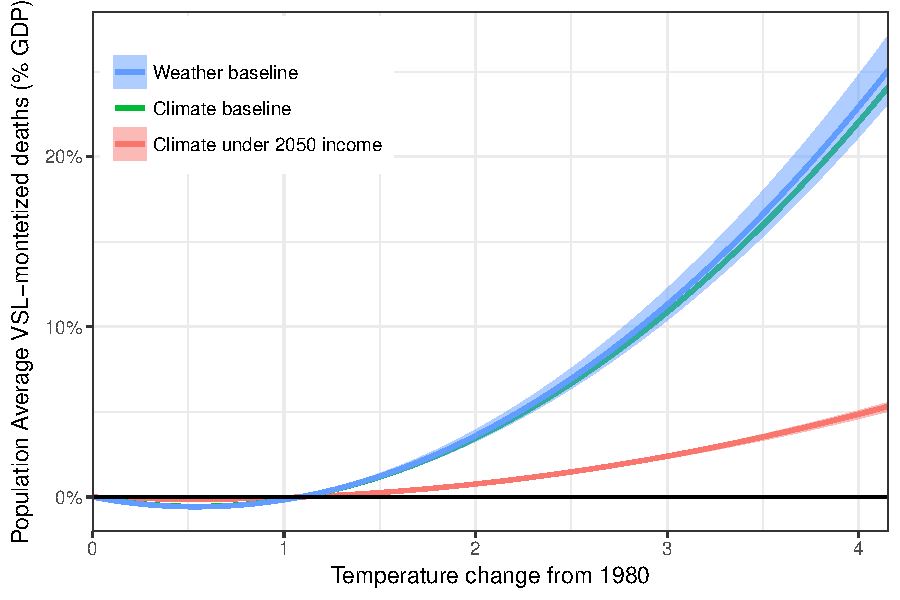
\includegraphics[width=\textwidth]{damagefunc2.pdf}
}

\frame{
\frametitle{Bayesian fitted parameters}

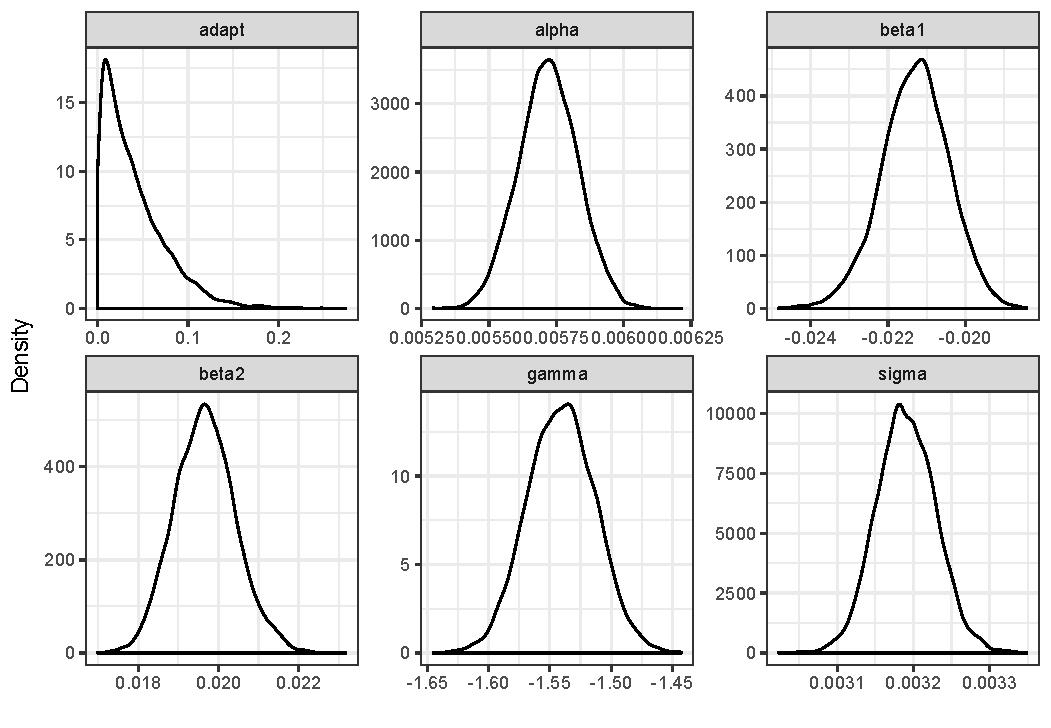
\includegraphics[width=\textwidth]{bayes.pdf}
}


\frame{
\frametitle{Results}

\begin{tiny}
\begin{tabular}{lllrrrrrrrr}
RCP & SSP & Monetization & 0 & 0.01 & 0.02 & 0.03 & 0.04 & 0.05 & 0.06 & 0.07 \\
4.5 & SSP4 & VSL ag02 popavg & 49.765215 & 20.090173 & 11.188628 & 7.319126 & 5.2335889 & 3.9565314 & 3.1067942 & 2.5073709 \\
4.5 & SSP4 & VSLY popavg & 27.076281 & 11.585834 & 6.923858 & 4.851441 & 3.7002694 & 2.9724734 & 2.4727046 & 2.1093082 \\
4.5 & SSP4 & VSLY scaled & 4.846833 & 2.353378 & 1.527805 & 1.128928 & 0.8938308 & 0.7389402 & 0.6293463 & 0.5477955 \\
4.5 & SSP4 & VSL ag02 scaled & 10.848195 & 5.175614 & 3.320996 & 2.429363 & 1.9066906 & 1.5647519 & 1.3247003 & 1.1474737 \\
4.5 & SSP5 & VSL ag02 popavg & 22.639750 & 12.790459 & 9.110520 & 7.113661 & 5.8206464 & 4.9042500 & 4.2186996 & 3.6866908 \\
4.5 & SSP5 & VSLY popavg & 11.801313 & 7.208263 & 5.423449 & 4.413440 & 3.7358821 & 3.2413275 & 2.8619107 & 2.5608733 \\
4.5 & SSP5 & VSLY scaled & 3.848509 & 2.133306 & 1.521382 & 1.197915 & 0.9917263 & 0.8470242 & 0.7393777 & 0.6560325 \\
4.5 & SSP5 & VSL ag02 scaled & 11.471691 & 5.608791 & 3.721099 & 2.799517 & 2.2450104 & 1.8726067 & 1.6050818 & 1.4037624 \\
8.5 & SSP4 & VSL ag02 popavg & 112.962731 & 41.333858 & 21.802857 & 13.955777 & 9.9695436 & 7.6319429 & 6.1235417 & 5.0814877 \\
8.5 & SSP4 & VSLY popavg & 54.144549 & 20.820391 & 11.622419 & 7.842783 & 5.8696309 & 4.6790999 & 3.8891723 & 3.3288767 \\
8.5 & SSP4 & VSLY scaled & 10.365246 & 4.535453 & 2.715188 & 1.892462 & 1.4381250 & 1.1560006 & 0.9663930 & 0.8312908 \\
8.5 & SSP4 & VSL ag02 scaled & 22.627928 & 10.012589 & 5.961467 & 4.101235 & 3.0711859 & 2.4350453 & 2.0115973 & 1.7132506 \\
8.5 & SSP5 & VSL ag02 popavg & 43.699053 & 21.802650 & 14.734155 & 11.293759 & 9.2161600 & 7.8077671 & 6.7840025 & 6.0041636 \\
8.5 & SSP5 & VSLY popavg & 20.489387 & 11.096381 & 7.938798 & 6.331466 & 5.3222833 & 4.6156765 & 4.0879440 & 3.6765711 \\
8.5 & SSP5 & VSLY scaled & 6.789311 & 3.387298 & 2.244069 & 1.682805 & 1.3488154 & 1.1277918 & 0.9711668 & 0.8546137 \\
8.5 & SSP5 & VSL ag02 scaled & 19.423931 & 8.974785 & 5.584819 & 3.984682 & 3.0697847 & 2.4871389 & 2.0886172 & 1.8013216 \\
\end{tabular}
\end{tiny}
}

\frame{
\frametitle{Calculating an SCC (one slide for MG)}

\begin{enumerate}
\item We estimate a global damage function: total monetized costs as they vary with temperature change from the baseline.
\begin{center}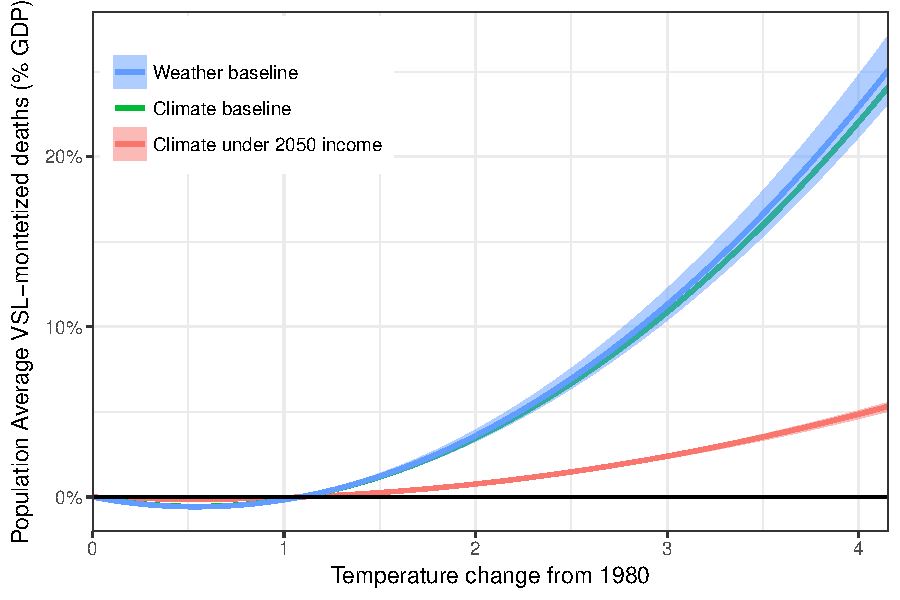
\includegraphics[width=.6\textwidth]{damagefunc2.pdf}\end{center}
\item The damage function includes the effect of temperature adaptation (minor here) and income adaptation (huge).
\item We calculate $(A)$ costs for each year according to an RCP scenario, and $(B)$ costs for a 1 tonne boost in 2017 above that scenario.
\item The SCC is the present discounted value of $(B) - (A)$.
\end{enumerate}
}

\section{Reduced-form estimation}
\frame{
\frametitle{Calculating an SCC}
Let $x_t$ be a stream of CO$_2$ emissions and $y_t$ be the stream of impacts.

Let $f(t)$ be an impulse response function which describes how a single GT jump in CO$_2$ produces a stream of impacts.  Then, $y_t = x_t \ast f(T)$, the result of a convolution.

\begin{enumerate}
\item We assume that each unit increase in CO2 has an impact that starts near 0, rises rapidly, and slowly decays.  It also varies with average global temperature $T$.
\item The entire stream of impacts from CO2 is the just the sum of scaled and translated copies of this impulse response.
\item We calculate the coefficients that define that impulse response.
\item We calculate the NPV of the impulse response.
\end{enumerate}
}

\frame{
\frametitle{A proposed structural form}

Suppose that $f(T) = \sum_{k=0}^K \left(\beta_{k0} + \beta_{k1} T\right) t^k e^{-t / \tau}$, where $\tau$ is the residence time of CO$_2$ in the atmosphere, 400 yr under IPCC or 77 yr under DICE.

Then,
\begin{align*}
y_t &= \alpha + \sum_{s=0}^\infty x_{t - s} \sum_{k=0}^K \left(\beta_{k0} + \beta_{k1} T_{t-s}\right) s^k e^{-s / \tau} + \epsilon_t \\
&= \alpha + \sum_{k=0}^K \beta_{k0} \sum_{s=0}^\infty x_{t - s} s^k e^{-s / \tau} + \sum_{k=0}^K \beta_{k1} \sum_{s=0}^\infty x_{t - s} T_{t-s} s^k e^{-s / \tau} + \epsilon_t
\end{align*}
 
This is just a weighted sum of recent CO$_2$ emissions as the predictors for a regression.
}

\frame{
\frametitle{Calculating an SCC}
We are interested in the discounted sum of impacts.  This can be calculated as,

\begin{align*}
SCC_t &= \sum_{u = 0}^\infty e^{-\delta u} y_{u}(\delta_u) \\
&= \sum_{u = 0}^\infty e^{-\delta u} \left[\sum_{k=0}^K \beta_{k0} \sum_{s=0}^\infty \mathbf{1}\{u-s = 0\} s^k e^{-s / \tau} +\right. \\
&\hspace{6em} \left.\sum_{k=0}^K \beta_{k1} \sum_{s=0}^\infty \mathbf{1}\{u-s = 0\} T_{u-s} s^k e^{-s / \tau}\right] \\
&= \sum_{u = 0}^\infty e^{-\delta u} \left[\sum_{k=0}^K \beta_{k0} u^k e^{-u / \tau} + \sum_{k=0}^K \beta_{k1} T_t u^k e^{-u / \tau}\right] \\
\end{align*}
}


\end{document}
